%% 
%% Copyright 2007-2020 Elsevier Ltd
%% 
%% This file is part of the 'Elsarticle Bundle'.
%% ---------------------------------------------
%% 
%% It may be distributed under the conditions of the LaTeX Project Public
%% License, either version 1.2 of this license or (at your option) any
%% later version.  The latest version of this license is in
%%    http://www.latex-project.org/lppl.txt
%% and version 1.2 or later is part of all distributions of LaTeX
%% version 1999/12/01 or later.
%% 
%% The list of all files belonging to the 'Elsarticle Bundle' is
%% given in the file `manifest.txt'.
%% 
%% Template article for Elsevier's document class `elsarticle'
%% with harvard style bibliographic references

%\documentclass[preprint,12pt]{elsarticle}

%% Use the option review to obtain double line spacing
%% \documentclass[preprint,review,12pt]{elsarticle}

%% Use the options 1p,twocolumn; 3p; 3p,twocolumn; 5p; or 5p,twocolumn
%% for a journal layout:
%% \documentclass[final,1p,times]{elsarticle}
%% \documentclass[final,1p,times,twocolumn]{elsarticle}
%% \documentclass[final,3p,times]{elsarticle}
%% \documentclass[final,3p,times,twocolumn]{elsarticle}
%% \documentclass[final,5p,times]{elsarticle}
\documentclass[final,5p,times,twocolumn]{elsarticle}

%% For including figures, graphicx.sty has been loaded in
%% elsarticle.cls. If you prefer to use the old commands
%% please give \usepackage{epsfig}

%% The amssymb package provides various useful mathematical symbols
\usepackage{amssymb}
%% The amsthm package provides extended theorem environments
%% \usepackage{amsthm}

%% Additional packages
\usepackage{epstopdf}
\usepackage[hyphens]{url}
\usepackage{xurl}
\usepackage[breaklinks]{hyperref}
\usepackage[hyphenbreaks]{breakurl}
\usepackage{wrapfig}

%% The lineno packages adds line numbers. Start line numbering with
%% \begin{linenumbers}, end it with \end{linenumbers}. Or switch it on
%% for the whole article with \linenumbers.
%% \usepackage{lineno}

\journal{Machine Learning}

\begin{document}

\begin{frontmatter}

%% Title, authors and addresses

%% use the tnoteref command within \title for footnotes;
%% use the tnotetext command for theassociated footnote;
%% use the fnref command within \author or \address for footnotes;
%% use the fntext command for theassociated footnote;
%% use the corref command within \author for corresponding author footnotes;
%% use the cortext command for theassociated footnote;
%% use the ead command for the email address,
%% and the form \ead[url] for the home page:
%% \title{Title\tnoteref{label1}}
%% \tnotetext[label1]{}
%% \author{Name\corref{cor1}\fnref{label2}}
%% \ead{email address}
%% \ead[url]{home page}
%% \fntext[label2]{}
%% \cortext[cor1]{}
%% \affiliation{organization={},
%%             addressline={},
%%             city={},
%%             postcode={},
%%             state={},
%%             country={}}
%% \fntext[label3]{}

\title{Towards Automated Bias Detection and Mitigation in Machine Learning}

%% use optional labels to link authors explicitly to addresses:
%% \author[label1,label2]{}
%% \affiliation[label1]{organization={},
%%             addressline={},
%%             city={},
%%             postcode={},
%%             state={},
%%             country={}}
%%
%% \affiliation[label2]{organization={},
%%             addressline={},
%%             city={},
%%             postcode={},
%%             state={},
%%             country={}}

\author{Alfa Yohannis, Dimitris Kolovos}

\affiliation{organization={Department of Computer Science, University of York},%Department and Organization
%            addressline={}, 
            city={York},
%            postcode={}, 
%            state={},
            country={United Kingdom}}

\begin{abstract}
Models produced by machine learning are not guaranteed free from bias, particularly when trained and tested with data produced in discriminatory environments. The bias can be unethically acceptable, especially when the data contains sensitive attributes, such as sex, race, age, etc. Some approaches have contributed to mitigating such bias by providing bias metrics and mitigation algorithms, and they are already supported by most fair machine learning toolkits. FairML brings a model-based approach to improve the fairness of machine learning by levelling up the abstraction and automatically generating the code and reports of bias measurement and mitigation.
\end{abstract}

%%Graphical abstract
\begin{graphicalabstract}
%\includegraphics{grabs}
\end{graphicalabstract}

%%Research highlights
\begin{highlights}
\item Research highlight 1
\item Research highlight 2
\end{highlights}

\begin{keyword}
%% keywords here, in the form: keyword \sep keyword

%% PACS codes here, in the form: \PACS code \sep code

%% MSC codes here, in the form: \MSC code \sep code
%% or \MSC[2008] code \sep code (2000 is the default)

\end{keyword}

\end{frontmatter}

%% \linenumbers

%% main text
\section{Introduction}
\label{sec:introduction}
The use of machine learning is pervasive nowadays, from personal daily activities, such as face recognition for authentication and voice processing when talking to smart assistants (e.g., Alexa, Siri), to performing sensitive, ethical tasks, such as predicting criminals and classifying profiles for loans. While machine learning does bring efficiencies, models produced by machine learning are not guaranteed free from bias, particularly when trained and tested with data produced in discriminatory environments. The bias can be unethically acceptable, particularly when it touches sensitive attributes, such as sex, race, age, etc., and cause unfairness. 

In 2016, an algorithm for predicting recidivism was found produced high false negative rate for white people and high false positive rate for black people \cite{angwin2016machine}. Some commercial face recognition services were also found having significant lower accuracy on darker-skin females \cite{buolamwini2018gender}. Moreover, A job platform was found to rank qualified female candidates far lower than qualified male candidates even though they have similar properties \cite{lahoti2019ifair}. These are some of many other instances that show biases in machine learning can promote unfairness. 

Some approaches have contributed to the mitigation of such biases by providing metrics []  and algorithms [] to measure and mitigate biases. Some toolkits do exist to allow users to implement such metrics and algorithms (see Table \ref{tab:bias-mitigation-toolkits}).
However, these toolkits come with different methodological approaches and capabilities which users need to understand so that they can decide which toolkits are best for certain scenarios~\cite{lee2021landscape}.  

Data scientists usually work using their intuitions to narrow down the number of combinations of algorithms, parameters, and other factors in order to find the best models for given goals, datasets, and domains \cite{muller2016introduction}. After that, with lots of experimentation and trial and error \cite{byrne2017development}, they have to go through all the narrowed combinations and test the produced models to identify which models are the best. Moreover, regardless of the availability of machine learning libraries, data scientists have to craft the search process from scratch in general/statistical programming languages (e.g, Python, R).

Model-Driven Sofware Development (MDSE) leverage the abstraction of software development by hiding technical details of implementation that can be automated \cite{brambilla2017model}. Thus, users can focus on important aspects through the use of simpler modelling languages, and the target implementation can be automatically generated, which in turn improve productivity \cite{volter2013model}. The use of MDSE would benefit data scientists since it allows them to search for the best bias mitigation methods for given cases at a higher abstraction level. They also do not have to code the implementation of the search process in general/statistical programming languages since it can be automatically generated and then fine tuned later on. 

The contribution of this research is FairML, a tool that implements MDSE approach to model and automate measuring and mitigating biases in machine learning. 
\begin{enumerate}
\item FairML raises up the abstraction of bias measurement and mitigation so that users can configure their bias mitigation model in YAML (YAML Ain’t Markup Language), a human-friendly declarative language \cite{evans2017yaml}, without having to code in general/statistical programming languages.
\item FairML supports certain degree of expressiveness which allows users to experiment with different kinds of bias metrics, bias mitigation algorithms, datasets, classifiers, and their parameters to find the best of their combinations that reduces biases but with acceptable accuracy.
\item It automatically generates Python and Jupyter Notenbook files which users can execute to run measure and mitigate biases on given datasets. All generated files are modifiable and extensible for fine tuning and further development.
\end{enumerate}



\section{Bias in Machine Learning}
\label{sec:bias_in_machine_learning}

\subsection{Definitions and Examples}
\label{sec:definitions_and_examples}

Fairness in defined as ``the absence of any prejudice or favoritism toward an individual or
group based on their inherent or acquired characteristics'' \cite{mehrabi2021survey}.
The absence of fairness can be caused by bias which is a systematic error or distortion from the true state of affairs due to flaws in data collection and processing, study design, analysis, and interpretation \cite{oxford2022bias}. 
The unfairness happens when biases put privileged groups at the advantaged position against unprivileged groups \cite{bellamy2018ai}. 
Bias can also be caused by negative discrimination if the distinction made is due to intentional or unintentional stereotyping and prejudice based on sensitive attributes (race, age, sex, etc.) \cite{mehrabi2021survey,chen2019fairness}. 






A Survey on Bias and Fairness in Machine Learning

It has been found in 2016 that COMPAS, the algorithm used for recidivism prediction produces much higher false positive rate for black people than white people \cite{angwin2016machine}.

XING, a job platform similar to Linked-in, was found to rank less qualified male candidates higher than more qualified female candidates \cite{lahoti2019ifair}.

Publicly available commercial face recognition online services provided by Microsoft, Face++, and IBM respectively are found to suffer from achieving much lower accuracy on females with darker skin color \cite{buolamwini2018gender}.

\subsection{Bias Metrics}
\label{sec:bias_metrics}



Statistical parity Difference \cite{dwork2012fairness,bellamy2018ai} is a metric computed as the difference of the rate of favourable outcomes received by the unprivileged group to the privileged group. The ideal value of this metric is 0. Fairness for this metric is between -0.1 and 0.1.

Equal Opportunity Difference \cite{bellamy2018ai} is a metric computed as the difference of true positive rates between the unprivileged and the privileged groups. 
The true positive rate is the ratio of true positives to the total number of actual positives for a given group. The ideal value is 0. A value of $<$ 0 implies higher benefit for the privileged group and a value $>$ 0 implies higher benefit for the unprivileged group. Fairness for this metric is between -0.1 and 0.1.

Average Odds Difference \cite{bellamy2018ai} is a metric computed as average difference of false positive rate (false positives / negatives) and true positive rate (true positives / positives) between unprivileged and privileged groups.
The ideal value of this metric is 0. A value of $<$ 0 implies higher benefit for the privileged group and a value $>$ 0 implies higher benefit for the unprivileged group.
Fairness for this metric is between -0.1 and 0.1

Disparate Impact \cite{feldman2015disparate,bellamy2018ai} is a metric computed as the ratio of rate of favourable outcome for the unprivileged group to that of the privileged group.
The ideal value of this metric is 1.0 A value $<$ 1 implies higher benefit for the privileged group and a value $>$1 implies a higher benefit for the unprivileged group.
Fairness for this metric is between 0.8 and 1.25.

5. Theil Index \cite{conceicao2000theyoung,bellamy2018ai}
Computed as the generalized entropy of benefit for all individuals in the dataset, with alpha = 1. It measures the inequality in benefit allocation for individuals.
A value of 0 implies perfect fairness. Fairness is indicated by lower scores, higher scores are problematic.


 Fairness Measures (Zehlike et al., 2017), for example,
provides several fairness metrics, including difference of
means, disparate impact, and odds ratio. A set of datasets
is also provided, though some datasets are not in the pub-
lic domain and need explicit permission from the owners
to access/use the data. Similarly, FairML (Adebayo, 2016)
provides an auditing tool for predictive models by quantify-
ing the relative effects of various inputs on a models predic-
tions. This, in turn, can be used to assess the models fair-
ness. FairTest (Tram`

er et al., 2017), on the other hand, ap-
proaches the task of detecting biases in a dataset by check-
ing for associations between predicted labels and protected
attributes. The methodology also provides a way to iden-
tify regions of the input space where an algorithm might
incur unusually high errors. This toolkit also includes a
rich catalog of datasets. Aequitas (Stevens et al., 2018) is
another auditing toolkit for data scientists as well as pol-
icy makers; it has a Python library as well as an associated
web site where data can be uploaded for bias analysis. It
offers several fairness metrics, including demographic or
statistical parity and disparate impact, along with a ”fair-
ness tree” to help users identify the correct metric to use for
their particular situation. Aequitas’s license does not allow


AI Fairness 360

commercial use. Finally, Themis (Galhotra et al., 2017) is
an open source bias toolbox that automatically generates
test suites to measure discrimination in decisions made by
a predictive system.

\subsection{Bias Mitigation}
\label{sec:bias_mitigation}

A handful of toolkits address both bias detection as well
as bias mitigation. Themis-ML (Bantilan, 2018) is one
such repository that provides a few fairness metrics, such
as mean difference, as well as some bias mitigation algo-
rithms, such as relabeling (Kamiran \& Calders, 2012), ad-
ditive counterfactually fair estimator (Kusner et al., 2017),
and reject option classification (Kamiran et al., 2012). The
repository contains a subset of the methods described in the
paper. Fairness Comparison (Friedler et al., 2018) is one of
the more extensive libraries. It includes several bias detec-
tion metrics as well as bias mitigation methods, including
disparate impact remover (Feldman et al., 2015), prejudice
remover (Kamishima et al., 2012), and two-Naive Bayes
(Calders \& Verwer, 2010). Written primarily as a test-bed
to allow different bias metrics and algorithms to be com-
pared in a consistent way, it also allows the addition of ad-
ditional algorithms and datasets.

\section{Model-based Software Development}
\label{sec:model_based_software_development}
Model-Driven Sofware Development (MDSE) is a development paradigm of software in which models are used as the primary artefacts to drive the process of software development. The models are used as bases/references to (semi)automatically generate the target software \cite{brambilla2017model}. MDSE aims for a productive environment by speeding up development through artefact generation and managing complexity by raising up abstraction level in the form of simpler modelling languages \cite{volter2013model}. 

\section{Toolkit Selection}
\label{sec:toolkit_selection}

Lee et al. \cite{lee2021landscape} analysed the landscape of open source toolkits in algorithmic ethics particularly for fairness in machine learning. Based on the criteria that a toolkit is 1) open source, 2) likely to be used by practitioners, 3) implementing fairness-related methodology and through a focus group discussion of data scientists, they eventually selected 6 toolkits -- Aequitas\cite{saleiro2019aequitas}, Google What-If\cite{googlewhatif2020}, Scikit-fairnet/scikit-lego \cite{scikitfairness2022,scikitlego2022}, Fairlearn\cite{bird2020fairlearn}, and IBM AI Fairness 360 \cite{bellamy2018ai} -- as the objects their analysis.  

From these the six toolkits, we evaluate them again to examine if they are applicable to be integrated into our model-based approach. The selected toolkits would be used in the generated code to implement bias mitigation. The main criteria for the selection are 1) it should be open source, 2) it should support bias mitigation, 3) it provides Application Programming Interface (API) to be programmable and integrated into model-based approach, and 4) it supports various bias measurements and mitigation algorithms to enable users to find the best bias mitigation strategies. 

The first criterion is met by all of the toolkits, since they are all open source projects. We excluded Aequitas due to its inability to perform bias mitigation (second criterion); it only supports bias measurement. We also removed Google What-If since it does not have API\footnote{\url{https://groups.google.com/g/what-if-tool/c/zw4Rk5kxPIM}} to be integrated with other applications (third criterion); its customisation is limited to custom prediction function\footnote{\url{https://pair-code.github.io/what-if-tool/get-started/}}. Compared to the rest toolkits, IBM AI Fairness 360 has the most complete features -- it claims it has at least 10 state-of-the-art bias mitigation algorithms and 77 bias metrics\footnote{\url{https://aif360.mybluemix.net/}} -- while Fairlearn and Scikit-fairness/lego come second and third \cite{lee2021landscape}, and all meet the fourth criteria. Thus, we use the four toolkits in our domain analysis prior designing our solution.

%They also identified that there was a lack of consistency between the toolkits in their methodological approaches, and therefore users need to understand them at first before they can use the toolkits properly to meet goals.

\begin{table*}[]
	\centering
	\caption{Toolkits for bias mitigation in machine learning.}
	\label{tab:bias-mitigation-toolkits}
	\begin{tabular}{p{.15\textwidth}p{.39\textwidth}p{.39\textwidth}}
		\hline
		\multicolumn{1}{c}{\textbf{Toolkit}}                                   & \multicolumn{1}{c}{\textbf{Website}}                                                                                                  & \multicolumn{1}{c}{\textbf{Repository}}                                                                                     \\ \hline
		Fairlearn                                                              & \url{https://fairlearn.org}                                                                                                                 & \url{https://github.com/fairlearn/fairlearn}                                                                                      \\
		Google What-If                                                         & \url{https://pair-code.github.io/what-if-tool}                                                                                              & \url{https://github.com/pair-code/what-if-tool}                                                                                   \\
		Scikit-fairness, Scikit-lego & \url{https://scikit-fairness.netlify.app}, \url{https://scikit-lego.readthedocs.io/en/latest/index.html} & \url{https://github.com/koaning/scikit-fairness},  \url{https://github.com/koaning/scikit-lego} \\
		IBM AI Fairness 360                                                    & \url{https://aif360.mybluemix.net}                                                                                                          & \url{https://github.com/Trusted-AI/AIF360}                                                                                        \\ \hline
	\end{tabular}
\end{table*}



\section{Domain Analysis}
\label{sec:domain_analysis}

In order to model bias mitigation in machine learning, important constructs and workflows of the domain should be accommodated by the model \cite{volter2013model}. Usually, interviewing the experts in the field is the common option to capture the constructs and workflows. However, this can be challenging particularly in research or development with limited resources (e.g., low fund, tight schedules, expert availability). Therefore, we opted for document analysis as documents contain information to understand the objects of interests \cite{bowen2009document}. As showcases, Poncin et al. \cite{poncin2011process} and Rogers et al. \cite{rogers2015using} analysed code repositories and existing documentation to understand software development and maintenance processes. Thus, we analyse the code repositories and documentations of some bias mitigation toolkits in Table \ref{tab:bias-mitigation-toolkits} in order to understand their use and implementation in mitigating bias, with an assumption that they reflect bias mitigation in the real world. Our domain analysis aimed to identify constructs and workflows (their execution orders) in demos, tutorials, and examples, including identifying all the necessary dependencies required by the constructs, such as parameters, classes, functions, initialisation, etc.

\subsection{Constructs}
\label{sec:constructs}
Model-driven approach requires us to identify important constructs so that users only deal with these constructs when constructing models thus reducing complexity. The important constructs identified through our analysis of the toolkits' repositories are as follows. 

Scikit-fairness consists of three modules

\subsection{Workflows}
\label{sec:workflows}

\begin{figure}
	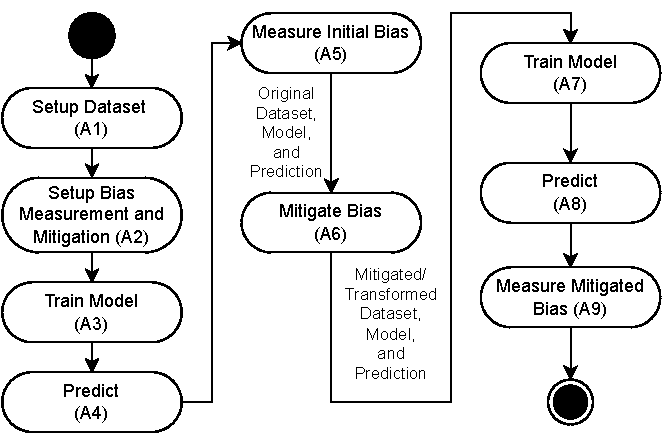
\includegraphics[width=\linewidth]{figures/workflow}
	\caption{The workflow of bias mitigation commonly performed using the toolkits in Section \ref{sec:toolkits}.}
	\label{fig:workflow}
\end{figure}

Our analysis found that, in general, all the toolkits perform the workflow presented in Figure \ref{fig:workflow}. Bias mitigation usually starts with setting up datasets (Action A1). In the action, users define the source of every dataset which is commonly a CSV file. They also profile each dataset to determine which attributes are the target/predicted attribute (including the favourable class in the attribute) and the sensitive attributes (including the privileged and unprivileged classes in the attributes).

In Action A2, users define the datasets and classifiers for model training. The training, validation, and test datasets are also set here, whether they are all come from different datasets or the same dataset but split with different ratios. They also select the bias metrics and mitigation algorithms that will be applied to datasets, models, and prediction. 

Users then train models in Action A3. The training can extend to validation for tuning hyper-parameters to obtain the best models. After that, users make prediction in Action A4 to measure the original accuracies of the models. The obtained accuracies will be compared against the accuracies post bias mitigation.
Users can skip the training and prediction (A3 and A4) if they only mitigate bias in the datasets, and the accuracies of prediction are not in concern.

Next, users measure the initial biases of the datasets, models, and prediction in Action A5. The scores of initial biases are used as benchmarks later on in the comparison against the scores of mitigated biases (A9). The results are compared

In the \textit{Mitigate Bias} action (A6), users apply bias mitigation algorithms to the original datasets, models, and predictions producing their bias-mitigated/transformed versions. In Action A7, the transformed datasets are then used to train new models (models created from bias-mitigated datasets). Using these models, together with models transformed from the original models in Action A6, users make new predictions (A8). 

Finally, after mitigated in Action A6, biases are measured again in Action A9. The mitigated biases are then compared to the original biases obtained in Action A5.  Users then analyse the results to find the best models with mitigated biases and accuracy that fit with their purposes. Results can be presented in numbers, tables, and charts to help users to examine the effects of the bias mitigation and choose the best models. 



\subsection{Design}
\label{sec:design}

\subsection{Use Cases}
\label{sec:use_Cases}

\section{Evaluation}
\label{sec:evaluation}


\subsection{Internal Evaluation}
\label{sec:internal_evaluation}

\begin{enumerate}
	\item written code vs. generated code
	\item code generation speed
	\item \textbf{Expressiveness?} Can it express the demo and examples provided by the toolkits? Or simulate the experiments in other papers? Does it show similar results?
\end{enumerate}

\subsection{User Evaluation}
\label{sec:user_evaluation}

\begin{enumerate}
	\item \textbf{RQ1: Does FairML raise the abstraction of bias mitigation processes?}
	
	FairML raises the abstraction and reduces the complexity of defining bias mitigation as opposed to describing it in a general programming language, such as Python. 
	
	\item \textbf{RQ2: Is FairML expressive enough to define bias mitigation processes?}
	
	FairML/YAML is expressive enough to define my bias mitigation processes. 
	
	('expressive' can be: it covers the necessary constructs or vocabulary of bias mitigation, I could easily write down what is my mind to define my bias mitigation)
	
	\item \textbf{RQ2: Does FairML speed up the development of bias mitigation implementation?}
	
	FairML's automated generation of Python code/Jupyter notebook speeds up the development of my bias mitigation code.
	
	\item \textbf{RQ4: Does FairML improve productivity in mitigating biases?}
	
	FairML (will) improve(s) my productivity in mitigating biases.
\end{enumerate}

Adult Census Income Dataset\footnote{\url{https://archive.ics.uci.edu/ml/datasets/adult}}

German Credit Dataset\footnote{\url{https://archive.ics.uci.edu/ml/datasets/Statlog+\%28German+Credit+Data\%29}}

Compas ProPublica Recidivism\footnote{\url{https://github.com/propublica/compas-analysis}}

\section{Discussion}
\label{sec:discussion}

%\section{Related Work}
%\label{sec:related_work}

\section{Conclusions and Future Work}
\label{sec:conclusions_and_future_work}

Alfa \cite{cormen2009introduction}

%% The Appendices part is started with the command \appendix;
%% appendix sections are then done as normal sections
\appendix

\section{List of Constructs}
\label{sec:list_of_constructs}

\begin{enumerate}
	\item Dataset.
	\item Label or Predicted/Target Attribute.
	\item Favourable Class/Group.
	\item Protected/Sensitive Attribute.
	\item Privileged Group/Class.
	\item Unprivileged Group/Class.
	\item Bias Metric.
	\item Bias Mitigation.
	\item Classifier.
	\item Model.
	\item Prediction.
	\item Bias Mitigation Algorithm.
	\item Training.
	\item Test.
	\item Validation.
	\item Accuracy.
	\item Bias.
	\item Parameters.
\end{enumerate}

%% For citations use: 
%%       \citet{<label>} ==> Jones et al. [21]
%%       \citep{<label>} ==> [21]
%%

%% If you have bibdatabase file and want bibtex to generate the
%% bibitems, please use
%%
  \bibliographystyle{elsarticle-num-names} 
  \bibliography{references}

%% else use the following coding to input the bibitems directly in the
%% TeX file.

%\begin{thebibliography}{00}
%
%%% \bibitem[Author(year)]{label}
%%% Text of bibliographic item
%
%\bibitem[ ()]{}
%
%\end{thebibliography}
\end{document}

\endinput
%%
%% End of file `elsarticle-template-num-names.tex'.
